\documentclass{report}
\usepackage[utf8]{inputenc}
\usepackage[french]{babel}
\usepackage[T1]{fontenc}
\usepackage{listings} 
\usepackage{hyphenat}
\hyphenation{mathéma-tiques récu-pérer sta-tis-ti-que}
\renewcommand{\theequation}{\thechapter.\arabic{equation}}
\setcounter{chapter}{-1}

\title{Fonctionement de R}
\author{Arthur Fontes Coêlho Cicic}

\begin{document}

\maketitle


\chapter{Les bases de R}

D'après moi Les plus grosses difficultés de ce cours viennent de l'utilisation et de la compréhension de R alors je vais essayer de couvrir les concepts importants du fonctionnement de R dans ce chapitre en simplifiant le tout. Je vais peut-être rentrer dans des détails qui vont être inutiles pour certaines personnes qui sont familières avec d'autres langages de programmation ou qui s'en foutent de comment ça marche. Ce chapitre est pour ceux qui ne comprennent rien et/ou qui sont curieux. Je veux aussi ajouter que vous n'avez pas besoin d'expérience en programmation pour le cours donc pas de panique. Finalement tout ce qui vas être dit dans ce chapitre n'as pas été donné dans le cours ou à été dit indirectement par des documents disponibles sur le moodle alors si tu veux tu peux ne pas lire cette partie.

\section{Qu'est ce que t'as installé ?}

Je pars du principe que tu as suivi les instruction d'installation données par le prof et que tu as déjà plusieurs choses dans ta machine.

\begin{enumerate}
    \item Le langage de programmation R.
    \item L'environnement de développement intégré (IDE) RStudio
    \item Peut-être des librairies ("c'est outil surprise qui nous servira plus tard")
\end{enumerate}

Les librairies ou packages en anglais 
\begin{lstlisting}[frame=single] 
# Pour installer des libraires packages en anglais
install.packages("e1071")
install.packages("oii")
\end{lstlisting}


\begin{figure}[htp]
    \centering
    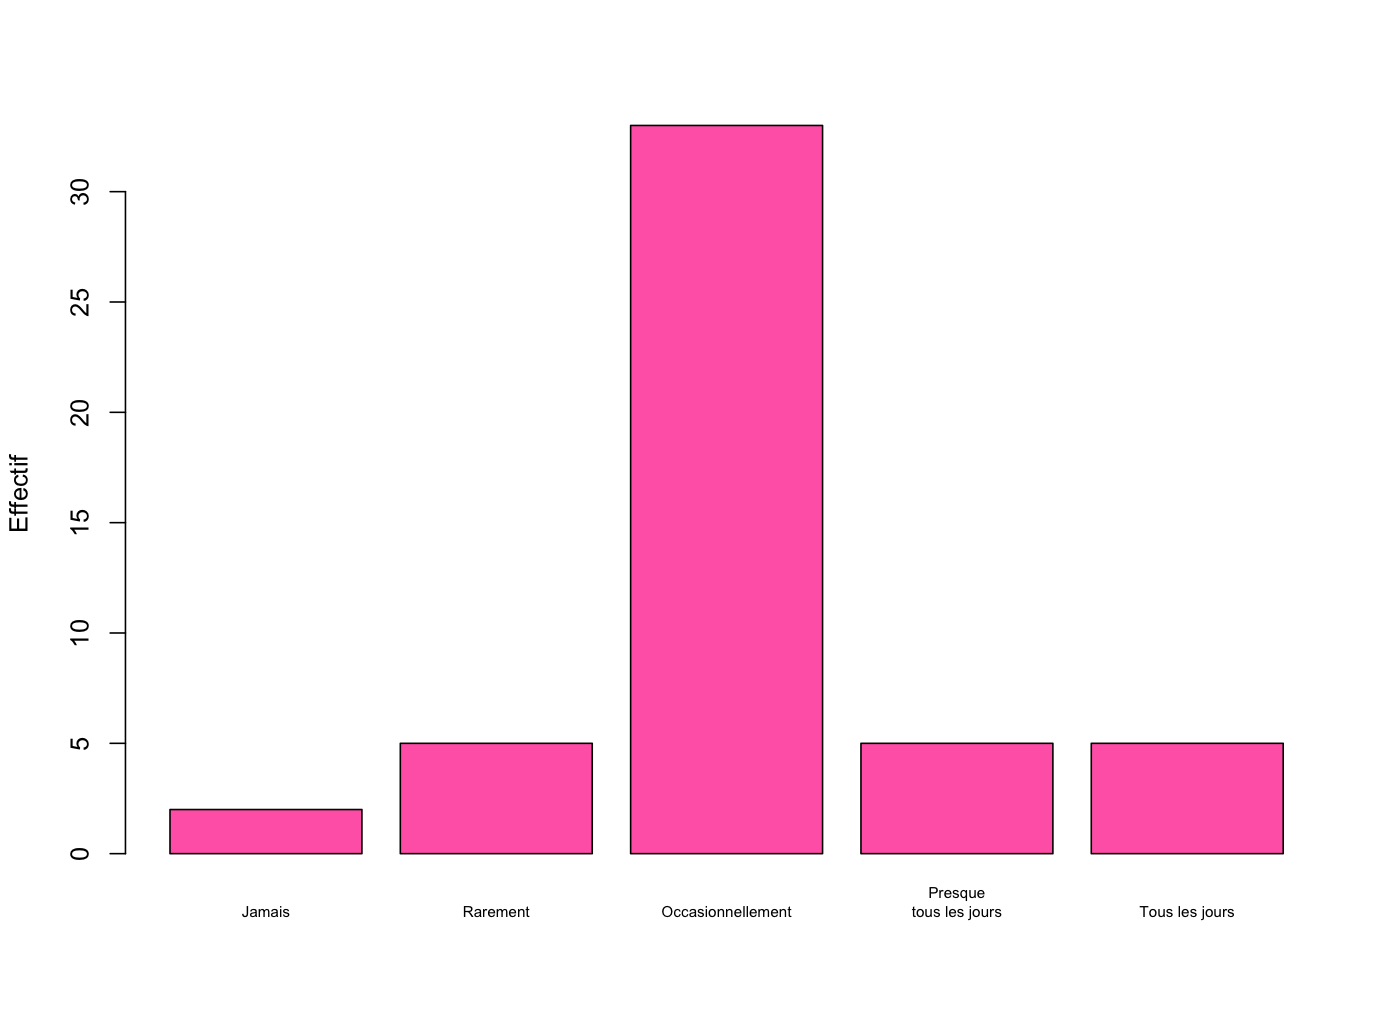
\includegraphics[width=12cm]{Images/diabaton.png}
    \caption{Résulatat de l'exemple}
    \label{fig:galaxy}
\end{figure}


qui comme expliqué précédemment prend pour arguments une valeur de départ, une valeur d'arrivée et une taille de saut pour créer un vecteur contenant une suite de nombre en fonction des valeurs définies.


\end{document}


